% Newman's contour: the circle |z|=R cut at Re z=-delta. Generated by a short script.
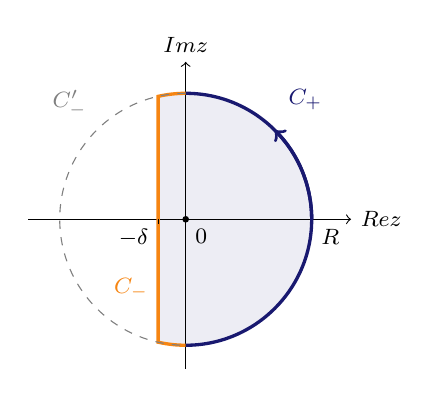
\begin{tikzpicture}[every node/.style={font=\footnotesize}]
\fill[MidnightBlue!8] (-0.35,-1.561) -- (-0.35,1.561) arc[start angle=102.64,end angle=-102.64,radius=1.6] -- cycle;
\draw[->] (-2.0,0)--(2.1,0) node[right] {$\operatorname{Re}z$};
\draw[->] (0,-1.9000000000000001)--(0,2.0) node[above] {$\operatorname{Im}z$};
\draw[MidnightBlue,very thick] (0,-1.6) arc[start angle=-90,end angle=90,radius=1.6];
\draw[MidnightBlue,very thick,->] (1.6,0) arc[start angle=0,end angle=45,radius=1.6];
\draw[BurntOrange,very thick] (0,1.6) arc[start angle=90,end angle=102.64,radius=1.6] -- (-0.35,-1.561) arc[start angle=-102.64,end angle=-90,radius=1.6];
\draw[gray,dashed] (0,1.6) arc[start angle=90,end angle=270,radius=1.6];
\node[MidnightBlue] at (1.520,1.520) {$C_+$};
\node[BurntOrange,left] at (-0.35,-0.880) {$C_-$};
\node[gray] at (-1.472,1.472) {$C_-'$};
\fill (0,0) circle (1.2pt) node[below right] {$0$};
\draw (-0.35,0)--(-0.35,-0.06); \node[below left] at (-0.35,0) {$-\delta$};
\node[below right] at (1.6,0) {$R$};
\end{tikzpicture}
